\chapter{Research Design and Shared Methodology}
\label{ch:methodology}

Chapter~\ref{ch:foundations} describes the technical components investigated in this thesis. Their utility depends on how they are implemented, trained, and tested.

This chapter details the methods employed in the studies. It covers the selection of the datasets and targets, the pairing of the observations, the training and testing of the models and the various ways in which uncertainty and reliability were assessed.

The methods follow the five criteria from the literature review. These criteria provide a common basis for the studies. Because the studies differ in data, labels, measurements, and computing resources, they address different subsets of the research questions.

\section{Research Design and Relationship to the Research Questions}

This thesis investigates multimodal methods for industrial monitoring, asking whether combining modalities improves prediction and how well the resulting methods perform. The research combines a literature review, dataset assessments, model development, comparative evaluations, and follow-up experiments. These experiments test whether particular representations and fusion techniques improve prediction under the conditions studied.

The studies are primarily exploratory. The research questions motivated the work, while available data, preliminary results, time, and accessible methods shaped its direction.

Later experiments addressed questions raised by earlier results and helped interpret those findings. Independent replication would require a separate evaluation of an architecture specified in advance.

The main comparisons are made within each study. Each representation or fusion method is tested against suitable reference models using the same target and assessment population.

The cross-dataset studies examine whether the methods remain useful across different tasks. Because the datasets differ in targets, observations, class balance, and evaluation procedures, their scores do not support a single cross-dataset ranking.

\subsection{Relationship Between the Research Questions and Case Studies}

The five main and supplementary studies address different aspects of the research questions: representation choice, the contribution of fusion, reliability, and evaluation measures beyond accuracy.

The PHM study constructs and predicts a continuous proxy for gear condition. Post-run photographs define the target, and the main regression models estimate it from machine-sensor data. The study addresses representation and fusion by comparing sensor representations and integrating sensor groups. It also examines proxy validity, regression performance, and grouped assessment. The reliability of visual–sensor fusion remains unresolved.

REASSEMBLE is the main experimental setting for evaluating multimodal fusion architectures. Its labelled completed actions, paired visual data, and machine-sensor data support comparisons of representations, single-modality predictors, static fusion, and context-based methods. The study evaluates CNN features, statistical features, PatchTST, pooling, and model adaptation. Its fusion and reliability tests examine feature- and prediction-level integration, known missing inputs, and controlled degradation. Grouped assessment, discrimination, calibration, uncertainty, and computational measurements provide context for interpreting the results.

MSM applies related methods to abnormal milling intervals. Its prediction target and controller measurements differ from REASSEMBLE’s completed-action classification task. The study compares visual and controller-based representations, unimodal and multimodal models, and performance under controlled input degradation. Grouped assessment, target sensitivity, ranking performance, and probability quality provide further methodological evidence.

ViFailback extends the investigation to complete manipulation episodes assessed across held-out tasks. It additionally examines whether transferring a visual representation learned on REASSEMBLE influences the predictive usefulness of visual information. Its completed experiments investigate frozen representations, donor transfer, bounded target-backbone adaptation, and prediction-level fusion. Task-disjoint assessment, class-specific ranking, and uncertainty address the evaluation question, while its corruption evaluation remains incomplete.

HANDOVER offers an additional comparison using video and force–torque data from labelled human–robot interaction trials. Its official assessment split supports evaluating single-modality predictors and fixed averaging. Missing participant-to-trial links prevent building participant-disjoint training predictions needed for the proposed learned-fusion comparison. The completed assessment also studies controlled sensor noise, visual blur, known input loss, and class-specific decisions.

The five studies examine different parts of the architecture problem. They do not establish performance in robotic welding; that requires data and evaluation from a welding study.

Figure~\ref{fig:research-workflow} relates the original welding objective and data-admission workflow to the five implemented studies.

\begin{figure}[htbp]
\caption{Workflow for Data Qualification and Model Evaluation}\label{fig:research-workflow}
\centering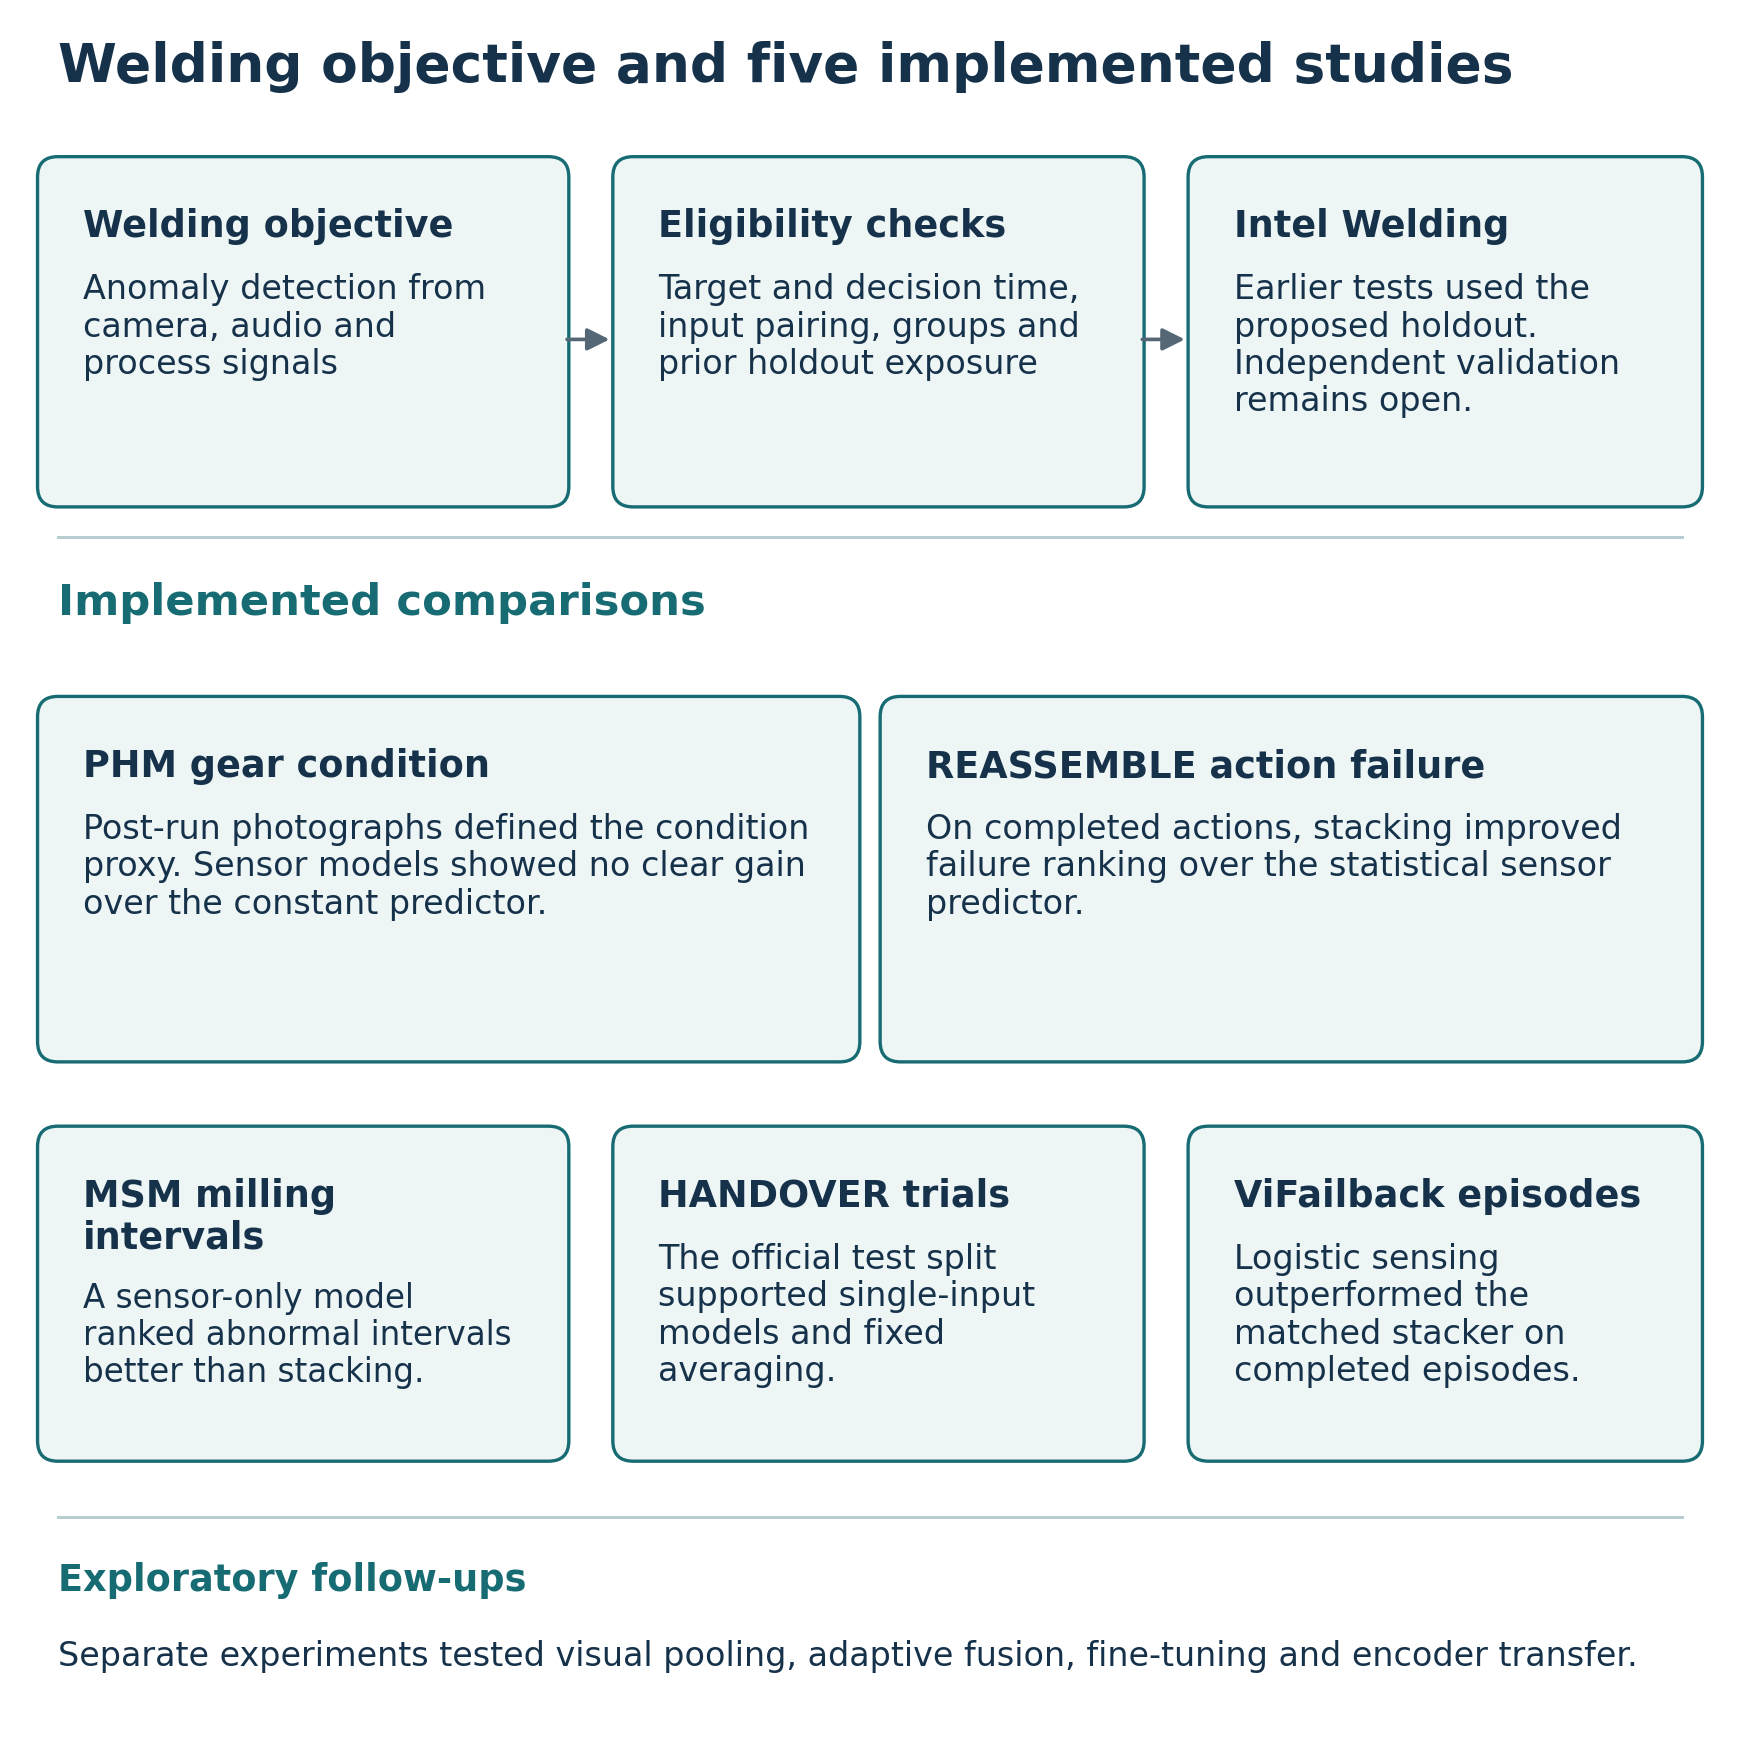
\includegraphics[width=\linewidth]{figures/research_workflow}
\displaynote{The five studies used different prediction targets. Each finding refers to the comparison within that study. The Intel holdout exposure refers to an earlier context audit, not a new trained-model test in the foundation review.}
\end{figure}

\subsection{Methodological Implementation of the Research Design Requirements}

Chapter 2 identified five requirements from the literature review. This chapter applies them to the multimodal monitoring methods investigated in the thesis.

R1 asks whether each study defines its outcome, explains where the target comes from, and specifies which observations are available when making predictions. Sections~\ref{sec:ch4-selection}--\ref{sec:ch4-targets} cover this through dataset selection, target creation, observation matching, and prediction-window definitions.

R2 asks whether the chosen representations fit the task. The chapter explains how each input is transformed, whether an encoder is pretrained or trained from scratch, and how aggregation, supervision, and training resources differ. The related procedures are detailed in Sections~\ref{sec:ch4-admission}, \ref{sec:ch4-fitting}, and~\ref{sec:ch4-boundaries}.

R3 asks whether fusion improves prediction beyond individual inputs. The comparisons in Sections~\ref{sec:ch4-assessment}--\ref{sec:ch4-metrics} use the same assessment observations and include single-modality and simple-fusion references. They also note differences in model size, calibration, and extra prediction steps where experiments allow.

R4 asks how models perform when inputs are missing, degraded, or collected under different conditions. These are separate tests, not interchangeable types of robustness. Section~\ref{sec:ch4-robustness} describes the tests done and the static or surviving-input references used for comparison.

R5 concerns the strength and limits of the evidence. Sections~\ref{sec:ch4-assessment}--\ref{sec:ch4-boundaries} cover dependence between samples, prior exposure to assessment data, metric and calibration choices, uncertainty, computational cost, reproducibility, and the information available during evaluation.

These requirements provide a framework for interpreting the completed studies; they do not imply that every experiment followed the same protocol from the outset.

Several consequential boundaries remain. PHM lacks an independent physical reference for its condition proxy. REASSEMBLE’s attribution of the full pooled fusion improvement is restricted by the absence of an independently refitted sensor-only second-stage control. MSM’s limited acquisition-date groups constrain uncertainty estimation. ViFailback’s corruption evaluation remains incomplete, and HANDOVER lacks the participant identifiers required for its proposed learned-fusion fitting procedure.

The empirical chapters keep these boundaries in place instead of treating incomplete requirements as if they were met.

Across the studies, the research progresses from dataset selection through comparisons of representations and fusion methods to reliability testing and interpretation. This sequence summarizes the programme; it does not imply that every study followed the same plan from the outset.

\section{Dataset Selection Criteria and Research Chronology}
\label{sec:ch4-selection}

A dataset is suitable for a particular study only when its available observations support both the prediction target and the planned comparison.

A public dataset may contain many measurements yet lack the labels needed for the prediction task. Another may have useful annotations but too few independent acquisition groups, or insufficiently matched observations, for a particular fusion experiment.

Datasets were assessed for accessible observations and documentation, a clearly interpretable target, and the availability of native labels or independent reference measurements.

The assessment also checked whether observations matched the prediction units, acquisition groups could be identified, outcome classes were represented, and the required processing and evaluation could be completed.

The relevance of each criterion depends on the planned comparison. A dataset may support target construction but lack the labels needed for supervised multimodal classification. It may also support fixed fusion of independently trained predictors while lacking the group identifiers required to train a second-stage fusion model without leakage.

The first robotic welding proposal came before the PHM and REASSEMBLE studies. The PHM investigation had already started when the renewed Intel Welding audit introduced more restrictions on the planned independent assessment.

REASSEMBLE then became the main experimental environment for comparing visual and machine-sensor representations and exploring different fusion architectures.

Later experiments looked into limitations found during the main studies. These included stronger sensor references, longer temporal-model training, different visual aggregation, encoder adaptation, context-conditioned fusion, and evaluation with external datasets.

The October research-alignment record kept the original four-question hierarchy after considering a narrower quality-gate investigation.

Although the empirical tasks changed, later studies continued to examine the same architectural research questions.

Additional dataset investigations, including PADERBORN, REBOOT, and other feasibility studies, are documented in Appendix~\ref{app:chronology}. These investigations are distinguished from completed principal experiments according to whether they produced an admissible comparison, a methodological finding, or an unresolved feasibility decision.

The experiments were not planned as one continuous sequence. Several follow-up comparisons were designed in response to earlier results and therefore remain exploratory.

The experimental reporting cutoff is 24 November 2026, with some saved-prediction verification done on 25 November 2026. Section~\ref{sec:ch4-reproducibility} documents the related source revisions, completion records, and evidence provenance.

\section{Intel Welding Feasibility Assessment and Scope Evolution}

The first research proposal considered robotic welding as the application for investigating process-aware multimodal fusion architectures.

The Intel Welding feasibility investigation examined dataset structure, observation readability, timing and session information, duplicate observations, and the suitability of the available partitions.

The associated foundation scripts inspect sample structure and assessment eligibility. Their recorded configuration turns off a final test because the proposed assessment population had already been examined during earlier context-related development.

The renewed audit also identified acquisition sessions spanning the supplied partitions. The results prevented the proposed population from being used as an untouched, independent confirmatory assessment.

Prior examination of an assessment population does not mean that every observation was used to train a model. However, it does limit the extent to which a later evaluation can be treated as an independent test of a fixed architectural hypothesis.

The retained dataset subset does not establish the entire original label mapping or a completed native multimodal welding classifier.

Consequently, the earlier context-related baseline records provide evidence concerning feasibility and design of the assessment rather than demonstrating that the proposed Transformer-based fusion architecture failed to predict welding quality.

The project documentation attributes the transition toward PHM and REASSEMBLE to an agreement with the supervisor reported by the researcher.

This transition preserves the principal research questions concerning representation learning, fusion mechanisms, reliability, and evaluation while changing the empirical tasks used to investigate them.

Success in adjacent industrial or robotic tasks does not establish successful welding-domain validation. An independent answer to the first welding application would require fresh welding observations, an appropriate weld-quality reference, and a reserved assessment population.

\noindent\textit{Internal implementation and decision evidence.} \EvidenceRef{E019}{inspect\_sample, audit\_split, main}, \EvidenceRef{E018}{}, \EvidenceRef{E003}{Section~3.1}.

\section{Dataset Admission and Preparation Checks}
\label{sec:ch4-admission}

Before an experiment, the available data were checked against the prediction task and assessment protocol.

The sample manifest records each prediction unit, target source, physical or operational group, input path, observation boundaries, available modalities, and any reason for exclusion.

The manifest also establishes the relationship between the source dataset population and the subset admitted to a particular experimental comparison.

Visual preparation checks examine whether observations can be decoded, whether sufficient frames are available, whether the image geometry is compatible with the extraction procedure, and whether the relevant process is represented within the viewing window.

An image may be technically readable yet provide no visible evidence of the target. Image quality and target visibility must therefore be assessed separately.

Sensor preparation checks examine channel ordering, physical units, timestamp consistency, missing observations, repeated measurements, and how interpolation or aggregation procedures are interpreted.

Resampling is particularly important when measurements are collected at diverse temporal resolutions or when sequences are transformed into a common action-progress representation.

These transformations must be recorded because they affect which properties of the source physical measurements remain available to the model.

Pairing checks whether observations from different sources belong to the same prediction unit. The mere presence of a video and a sensor file does not establish that they represent the same event or time interval.

Each admitted pair therefore requires a defined correspondence procedure.

Exclusions can influence the resulting class distribution and the difficulty of the assessment population. Removing corrupted observations or insufficiently represented failures may change the scientific interpretation of the comparison.

Counts before and after exclusion, together with the reasons for exclusion, are consequently retained where supported by the experimental records. Quarantined observations retain their original target annotations.

In MSM, timing-alias correction and grouping eligibility influence the admitted population. In ViFailback, duplicate or invalid telemetry records and video-readability failures affect the usable cohort.

These preparation checks establish technical eligibility. They do not independently validate semantic annotations, physical damage measurements, or the visibility of the relevant outcome within a camera observation.

Dataset qualification checks whether the target has an interpretable reference, the required measurements are usable, and the observations correspond to the same prediction unit. It also checks that assessment groups can be defined, outcomes are adequately represented, and the required processing and model fitting are computationally feasible.

Failure to satisfy a particular criterion may restrict the proposed comparison without invalidating every possible investigation of the dataset.

For example, insufficient participant information can prevent grouped learned-fusion fitting while still allowing an official fixed-model assessment. Similarly, the absence of an independent physical condition reference can restrict target interpretation while still permitting an investigation of proxy prediction.

These decisions operationalise R1 and establish the data-related conditions for the remaining research requirements.

\section{Target Provenance, Prediction Units, and Available Inputs}
\label{sec:ch4-targets}

A scientifically interpretable prediction task requires an explicit definition of what is predicted, how its reference value is obtained, and which observations are available at the intended prediction time.

A model’s predictive performance alone cannot establish that its target accurately represents the underlying physical or operational phenomenon.

This distinction is particularly relevant to the PHM investigation. Its image-derived candidate-area measure represents a provisional gear-condition proxy.

Predicting the proxy from machine-sensor observations measures agreement with the constructed target. It does not independently establish the accuracy of physical wear estimation, tooth-damage measurement, or remaining-useful-life prediction.

The robotic and machining studies use different operational outcomes.

In PHM, the principal prediction unit is a gear experiment run, and the target is a photograph-derived continuous condition proxy. REASSEMBLE predicts the recorded success or failure of completed robotic assembly actions. MSM predicts abnormal cutting within milling observation intervals. ViFailback predicts the recorded success or failure of complete manipulation episodes, while HANDOVER investigates binary outcomes associated with human–robot interaction trials.

The MSM investigation retains its declared mapping of native milling labels. Alternative mappings are considered through sensitivity analyses because changing the interpretation of a native label also changes the prediction task.

The meaning of the reported performance measures therefore depends on the target definition associated with each study.

\subsection{Observation Windows and Prediction Horizons}

The observation window determines the information available to the prediction model.

Sampling visual frames across a complete robotic action can provide information about its concluding state. Similarly, sensor statistics calculated over an entire milling interval describe observations collected throughout that interval.

These representations support retrospective assessment of condition or outcome. On their own, they do not show that a model can make a useful prediction before the operation is complete.

Prospective monitoring would require a defined decision time, causal preprocessing, a specified lead-time measure, and target annotations appropriate to the intended prediction horizon.

The retrospective experiments conducted in this thesis do not measure prospective warning time.

The distinction also influences computational interpretation. A model may produce a prediction rapidly after receiving its input, while acquiring the required observation window introduces additional delay.

The total time required for an operational prediction therefore includes both observation acquisition and the subsequent processing and inference stages.

\subsection{Contextual Information and Predictive Shortcuts}

Process identity, observation duration, time index, and other contextual variables can contain predictive information independently of the principal physical observations.

Such variables may provide useful context, but they can also introduce alternative explanations for apparent improvements.

For example, the extraction latency included in the PHM visual regression representation introduces a timing-related covariate alongside image-derived information.

Similarly, an action-conditioned fusion mechanism may exploit differences in failure prevalence between action categories. Its predictive improvement would not automatically establish that it recognised a deterioration in physical sensor quality.

Context-only references and constant-adjustment controls provide ways to investigate these alternative explanations where the corresponding comparisons are available.

The role of each contextual variable must therefore be interpreted in light of its relationship to the prediction target, acquisition procedure, and intended architectural function.

\section{Grouped Assessment, Data Splits, and Leakage Prevention}
\label{sec:ch4-assessment}

Reliable evaluation requires separating the observations used to develop a model from those used to assess its predictive performance.

Industrial and robotic observations often exhibit dependence because several samples originate from the same physical experiment, recording, task, machine, participant, or acquisition session.

Randomly partitioning individual observations may therefore place closely related samples into both development and assessment populations.

Such overlap can produce an evaluation that does not represent the intended level of generalization.

Grouped assessment prevents overlap at the specified dependence-group level. It does not, by itself, establish independence at higher physical or operational levels.

The appropriate grouping therefore depends on the scientific claim associated with the prediction task.

The principal PHM sensor protocol holds out complete gear experiments, while REASSEMBLE groups actions by recording. MSM examines experiment-based and acquisition-date groupings, and ViFailback separates manipulation tasks. HANDOVER retains the published official trial partitions.

The HANDOVER dataset publication describes its official participant-disjoint assessment. However, the available participant-to-trial correspondence does not permit independent reconstruction of that grouping or the construction of participant-disjoint inner training folds.

For MSM, an acquisition date may include multiple tools or operators. Physical equipment may also recur across dates. Consequently, date-disjoint assessment does not establish generalisation to an entirely new machine, factory, or installation.

A corresponding generalisation claim requires grouping information at the relevant physical level.

\subsection{Training-Side Preprocessing and Model Selection}

Within each outer assessment split, all data-dependent modelling operations must be considered part of model development.

These operations include feature scaling and normalisation, imputation parameters estimated from data, feature selection, supervised representation learning, hyperparameter selection, probability calibration, decision-threshold selection, and learned fusion fitting.

Separating these procedures from the assessment population is necessary because information can enter a prediction system through preprocessing or model selection even when the final classifier excludes the assessment labels.

Using cross-validation to select model configurations can produce optimistic error estimates if the same evaluation evidence is later used to report the selected performance \parencite{P004}.

More generally, leakage must be assessed through the complete modelling procedure, not only through the final training operation \parencite{P017}.

When a representation is derived using a fixed, generic pretrained encoder without target-specific supervision, its features may be cached before target-specific model fitting. However, any data-dependent normalisation, supervised adaptation, or feature selection must respect the corresponding permitted development population.

\subsection{Out-of-Fold Predictions and Learned Fusion}

Prediction-level stacking requires a second-stage training population containing the outputs of its first-stage predictors.

Using predictions generated from observations already included in first-stage fitting can provide the stacker with an unrealistically favourable description of branch performance.

Stacked generalisation therefore motivates constructing second-stage training inputs through cross-validated first-stage predictions \parencite{Ting1999Issues}.

In the grouped REASSEMBLE setting, the corresponding dependence group is the recording.

For each outer assessment split, the outer training population is partitioned into grouped inner fitting and prediction subsets. Branch models generate predictions for observations whose corresponding recordings were excluded from their fitting.

These predictions form an out-of-fold prediction bank used by subsequent training-side calibration, model-selection, and fusion-fitting procedures according to the relevant protocol.

The final selected branch models and prediction-level combination are then used to generate predictions for the designated outer assessment recordings.

The original REASSEMBLE stacker contains an additional methodological qualification.

Within each outer split, the stacker's internal validation reuses an out-of-fold prediction bank generated from the outer training recordings.

Although each predicted row originates from a branch that excluded its own recording, a branch used to generate a prediction for a stacker training row may have been fitted on recordings subsequently assigned to a stacker validation subset.

This introduces a dependency within the outer training population.

The outer assessment recordings remain excluded from fitting. The shared prediction bank therefore limits claims of strict independence at the deeper meta-validation stage without, by itself, establishing leakage from the outer assessment population.

This distinction matters: an evaluation may keep outer assessment data separate while using a less strictly nested procedure for internal model selection.

\noindent\textit{Internal implementation evidence.} \EvidenceRef{E004}{Section~15.4}.

\subsection{Assessment Cohort Reconciliation}

The validity of a comparative experiment also depends on whether the evaluated predictors use identical assessment observations.

Two reported results may refer to the same dataset while covering different samples, recordings, outcome classes, or preprocessing eligibility conditions.

The original REASSEMBLE assessment population contains 4,530 completed actions from 148 recordings, including 509 failures.

Its five outer assessment partitions collectively cover this population.

A later comparison involving 753 actions uses one of these previously examined outer partitions. It therefore provides additional evidence for a bounded experimental comparison but does not constitute a new independent external holdout.

An earlier summary identified this subset as containing 28 recordings. Reconciliation of the recorded sample and recording identifiers establishes that the population contains 26 recordings.

The assessment identities, rather than the earlier summary count, define the population associated with the comparison.

\noindent\textit{Internal cohort evidence.} \EvidenceRef{E052}{}.

\subsection{Historical Preprocessing Dependencies}

The principal PHM sensor protocol fits its normaliser separately within each training fold.

However, a separate four-arm diagnostic runner fits its normaliser before entering the loop that changes the held-out gear experiment.

In that diagnostic, observations from the held-out experiments therefore influence the fitted preprocessing transformation.

This limits interpreting the comparison as a strictly fold-isolated evaluation.

The principal PHM experiment and the four-arm diagnostic must consequently remain separate when reporting their procedures and interpreting their results.

A fully fold-isolated estimate for the four-arm diagnostic would require repeating the corresponding experiment under a revised preprocessing procedure. Such a repetition is not part of the completed evidence.

\subsection{Repeated Assessment Exposure}

Grouped assessment protects against specified forms of information overlap within individual model fits. It does not remove the consequences of repeatedly examining the same assessment population during exploratory research.

When later configurations are selected in response to previously observed assessment results, those results influence the research development process even if their observations remain excluded from the training of each subsequent model.

The REASSEMBLE follow-up investigations therefore provide informative controlled comparisons within an already examined population.

These follow-ups differ from a confirmatory experiment, which would specify all architectures, fitting conditions, primary metrics, and decision criteria before evaluating an independent assessment population.

This distinction also applies to uncertainty estimates calculated from the retained fitted predictions. Such estimates do not automatically account for the complete historical process through which the evaluated configurations were selected.

\section{Model Fitting, Selection, Calibration, and Threshold Procedures}
\label{sec:ch4-fitting}

Evaluating representation and fusion mechanisms depends on the procedures through which their parameters are estimated, and their predictions are converted into decisions.

Each empirical comparison therefore identifies its trainable components, initialisation procedure, preprocessing, candidate configurations, training budget, and relevant stopping or selection conditions.

The experimental programme includes original baseline comparisons, exploratory pilots, controlled follow-ups, and matched short-budget investigations.

Several more extensive experiments completed only a subset of their originally planned configurations. Their interpretation is restricted to the comparisons for which the required fitting and assessment stages were completed.

The prediction procedure distinguishes four operations: fitting model parameters, selecting a model, calibrating probabilities, and selecting a decision threshold.

\subsection{Model Fitting and Selection}

Model fitting estimates the parameters of the selected prediction architecture using its permitted training observations.

Model selection subsequently determines which representation, hyperparameter configuration, or fitting procedure is retained for assessment.

These operations can involve different data subsets and different criteria.

Equating the number of training epochs does not necessarily mean equivalent optimisation exposure if the configurations differ in batch size, available observations, early stopping, initialisation, or trainable components.

Similarly, a pretrained frozen representation and a scratch-trained temporal encoder receive different forms of prior information and allocate computational resources differently.

The evaluation therefore retains the actual fitting procedures associated with each comparison rather than treating equal epoch counts as a complete definition of experimental fairness.

\subsection{Probability Calibration}

Probability calibration concerns the relationship between predicted probabilities and observed outcomes.

A model can discriminate effectively between positive and negative observations while producing poorly calibrated probability estimates.

Calibration methods use development-side predictions and corresponding outcomes to adjust the numerical interpretation of prediction scores. Validation-based calibration can improve probability quality under appropriate conditions, but its effectiveness must be assessed rather than assumed \parencite{Guo2017Calibration}.

The principal REASSEMBLE branch calibrators use sigmoid logistic maps fitted to selected inner out-of-fold prediction scores.

The subsequent fusion mechanisms apply different probability transformations.

F2 introduces a fitted logistic map with a free intercept and separate branch coefficients. It does not include an additional post-stacker calibration stage in the recorded core implementation.

The original context-conditioned gates combine branch logits through normalised weights and apply a sigmoid to the resulting weighted value. They do not include a free final intercept or an additional post-gate calibrator.

These differences influence the numerical outputs of the evaluated prediction systems and can affect their discrimination and probability quality.

\subsection{Within-Fold Ranking and Pooled Prediction Scores}

The effect of a score transformation depends on the level at which predictions are evaluated.

A strictly increasing transformation preserves the ordering of observations within a fixed assessment population. Consequently, it preserves ranking-based metrics such as average precision and AUROC within that population, subject to numerical precision and tie handling.

When a sensor probability is transformed through a logistic function with a positive sensor coefficient, its ordering remains unchanged within the corresponding fold.

However, independently fitted transformations can differ between assessment folds.

When predictions from different folds are pooled, these transformations may change the relative ordering of observations originating from different folds, even though the ordering within each fold remains unchanged.

Consequently, pooled average precision may change even when the ranking within every individual fold remains unchanged.

This distinction is particularly relevant when evaluating learned fusion against a constituent unimodal predictor.

A comparison can involve both additional information from another prediction branch and an additional fitted transformation of the existing score.

Within-fold discrimination, pooled ranking, and probability calibration therefore represent distinct effects.

A matched sensor-only second-stage predictor provides an additional control for investigating the contribution of the fitted transformation. Where such a separately fitted control is unavailable, arithmetic analysis of the retained model can provide narrower evidence about the contribution of particular terms without resolving the complete attribution problem.

The corresponding REASSEMBLE saved-prediction investigation is presented in Chapter~6.

\subsection{Decision-Threshold Selection}

Binary classification requires a decision rule that converts prediction probabilities or scores into outcome labels.

Observations with prediction scores at or above the selected threshold are classified as positive, while those below the threshold are classified as negative.

The threshold influences the number of observations classified as positive and therefore changes sensitivity, specificity, precision, and false-positive behaviour.

The original implementation examines a threshold grid ranging from 0.01 to 0.99 using permitted training-side predictions and a specified selection objective, such as balanced accuracy.

A threshold selected in this way belongs to the experimental evaluation protocol. It is not necessarily an operationally optimal industrial alarm threshold.

Industrial decision-making may assign different costs to missed failures, false alarms, interruptions, or unnecessary maintenance. Establishing an operationally appropriate threshold would require information about these consequences and the intended monitoring application.

The empirical examinations therefore distinguish predictive discrimination from decisions obtained using the specified threshold-selection procedure.

\section{Metrics and Uncertainty Estimation}
\label{sec:ch4-metrics}

The evaluation metrics used throughout the thesis reflect the different prediction targets and scientific questions addressed by the empirical studies.

Regression error, classification discrimination, probability quality, and threshold-dependent decisions describe different properties of a prediction model.

Their interpretation also depends on the target definition, class distribution, assessment population, and aggregation procedure.

\subsection{Regression Metrics}

Regression performance is evaluated using errors between the predicted and observed continuous target values.

Mean absolute error describes the average absolute difference between predicted and observed target values. Root mean squared error calculates the square root of the average squared prediction error.

Both measures retain the units of the prediction target.

Mean absolute error describes the average magnitude of prediction deviations, while root mean squared error assigns greater influence to larger prediction errors through its squared-error formulation.

The coefficient of determination compares prediction error against the variation of the observed target values. It may become negative when the fitted predictor performs poorly relative to its reference denominator and can be unstable when the variation within an assessment group is limited.

In PHM, the physical interpretation of these metrics depends on the validity of the photograph-derived condition measure.

Low error establishes predictive agreement with the constructed target rather than independently verified physical damage estimation.

Tooth-level and run-level regression measurements are reported separately because they represent different prediction units and dependence structures.

\subsection{Classification Metrics}

Binary classification can be evaluated using threshold-dependent decisions and ranking-based performance measures.

Accuracy describes the proportion of correctly classified observations. Precision measures the proportion of positive predictions corresponding to actual positive outcomes. Recall measures the proportion of actual positives identified by the classifier.

Specificity measures the proportion of negative observations correctly classified, while balanced accuracy gives equal importance to sensitivity and specificity.

F1 combines precision and recall through their harmonic mean.

These threshold-dependent measures describe the decisions produced by a specified classification threshold.

Ranking-based measures instead examine how well the model orders positive and negative observations across possible thresholds.

The area under the receiver operating characteristic curve, AUROC, evaluates discrimination between positive and negative observations.

Average precision summarises the precision–recall relationship and provides a useful measure for classification tasks involving imbalanced outcomes. Precision–recall analysis can reveal aspects of predictive performance that are less apparent from ROC-based interpretation when one outcome class is relatively uncommon \parencite{Saito2015PrecisionRecall}.

Macro average precision additionally gives equal importance to the class-specific average precision values. Probability quality is examined through measures such as the Brier score and expected calibration error, which respectively characterise squared probability error and discrepancies between confidence and observed outcome frequencies.

The metrics available for each study depend on its target, prediction outputs, and completed evaluation protocol.

Their inclusion in the shared methodological framework does not imply that every metric was calculated for every experiment.

\subsection{Average Precision and Outcome Prevalence}

The principal classification ranking metric is average precision, calculated using the \texttt{average\_precision\_score} implementation.

Average precision summarises the precision–recall relationship by weighting precision values by their corresponding increments in recall.

This formulation is distinct from estimating the area under a precision–recall curve through trapezoidal numerical integration.

Average precision depends on the prevalence of the designated positive class.

If a binary predictor assigns the same score to every observation, its average precision equals the positive-class prevalence in the assessment population.

Thus, the same absolute average precision value can have different implications under different outcome distributions.

A high failure average precision may provide limited evidence of discrimination when failure already represents the majority of the evaluated observations.

This principle is particularly relevant to the ViFailback assessment, where failure constitutes more than 85\% of the principal eligible population.

Reporting only failure average precision can therefore obscure the model’s ability to identify successful outcomes.

Where both outcomes are relevant, class-specific average precision can be calculated separately for success and failure. Their binary macro average is obtained by calculating the arithmetic mean of these two class-specific values.

The macro average assigns equal importance to the two class-specific ranking measures rather than allowing the majority outcome alone to determine the reported summary.

For a constant-score binary predictor, the both-class macro average precision reference equals 0.5 when both outcome classes are present.

The interpretation of class-specific and macro-average precision must nevertheless retain the associated target definition and assessment population.

REASSEMBLE principally reports failure average precision. MSM reports abnormal-cutting average precision. ViFailback additionally reports both-class macro average precision.

These are distinct evaluation quantities and must not be interpreted as directly comparable numerical measures of architectural performance across the datasets.

\subsection{Metric Aggregation Across Folds and Seeds}

Grouped cross-validation produces predictions from separately fitted models associated with different assessment partitions.

Performance can be summarised through metrics calculated within individual folds, averages of those fold-level metrics, or metrics calculated after combining the held-out predictions.

Mean-fold average precision is calculated by obtaining the average precision for each assessment fold and subsequently averaging those values.

Pooled average precision instead combines the corresponding held-out prediction vectors and calculates average precision over the combined population.

Because average precision is nonlinear, these aggregation procedures generally produce different numerical results.

The pooled value can also depend on how scores align across separately fitted fold models.

The original REASSEMBLE primary comparison reports pooled failure average precision across its held-out recording partitions.

MSM reports abnormal-cutting average precision averaged over seed-specific pooled predictions.

ViFailback distinguishes failure average precision, success average precision, and their both-class macro average.

Reported seed variation and fold variation must also remain separate. Different random initialisations or fitting seeds represent another source of experimental variation rather than additional independently acquired assessment observations.

All reported comparisons therefore retain the metric definition, positive-class convention, aggregation procedure, seed configuration, and assessment population associated with the original result.

\subsection{Probability Quality and Calibration}

Probability-based assessment examines whether numerical prediction probabilities provide a useful description of observed outcome frequencies.

The Brier score measures the average squared difference between predicted probabilities and observed binary outcomes.

Unlike ranking-based measures, the Brier score is sensitive to the numerical probability values assigned to observations.

Proper scoring rules provide a principled basis for assessing probability forecasts rather than only their ranking or thresholded decisions \parencite{P055}.

Expected calibration error provides a complementary description based on discrepancies between predicted confidence and observed outcome frequencies across probability bins.

Its interpretation depends on the number and construction of bins, the definition of confidence, and the available observations within each bin.

A classifier with strong ranking performance may still assign poorly calibrated probabilities. Conversely, a model with improved probability error may not provide better discrimination.

The evaluation therefore distinguishes these properties rather than treating calibration, average precision, AUROC, and threshold-dependent classification as interchangeable indicators of reliability.

Probability calibration can also change under altered input conditions. Evidence from clean-data calibration must therefore be interpreted separately from probability quality under degradation or distribution shift \parencite{P008}.

\subsection{Paired Model Comparisons and Uncertainty Estimation}

The scientific interpretation of a performance difference requires consideration of its magnitude and associated uncertainty.

For two prediction models evaluated on the same observations, a paired comparison can be obtained by subtracting the average precision of the reference model from that of the investigated model.

A positive difference indicates higher average precision for the investigated model on that assessment population, while a negative difference indicates higher average precision for the reference model.

The paired construction retains the common observations and corresponding outcomes for the two models. This supports a more direct comparison than interpreting their performance estimates independently.

The uncertainty analyses use cluster-based bootstrap procedures where supported by the retained experimental records.

A cluster bootstrap resamples the specified dependence groups with replacement, rather than resampling individual observations independently. It then recalculates the paired metric difference for each resampled population.

The core REASSEMBLE reports use 2,000 recording-level bootstrap replicates.

A PHM report uses 10,000 run-cluster bootstrap replicates over 20 runs from three gear experiments.

The latter resampling procedure requires particular care because runs from the same gear experiment may retain higher-level dependence. Run-level resampling does not automatically capture all dependence between observations originating from the same physical experiment.

The reported interval remains associated with the original run-cluster procedure, and its interpretation must retain this restriction.

Increasing the number of bootstrap replicates reduces the numerical variability of the estimated resampling distribution. It does not increase the number of independently acquired physical experiments.

Similarly, the MSM date-cluster intervals rely on a particularly limited population of five acquisition dates. Their interpretation remains conditional on those groups and the recorded fitted models.

Cross-validation folds also share training observations. They should therefore not be treated as independent experimental replications when calculating uncertainty. \textcite{Bengio2004CVVariance} establish the limitations of universally unbiased variance estimation for k-fold cross-validation, supporting caution when constructing uncertainty estimates from overlapping training populations.

The retained bootstrap intervals characterise uncertainty under the selected resampling unit and fitted prediction vectors.

They do not automatically include uncertainty associated with retraining, additional model-selection procedures, repeated assessment exposure, or future industrial installations.

An uncertainty interval containing zero does not establish that two methods are equivalent. Likewise, a positive point estimate does not, by itself, establish a practically meaningful or reproducible improvement.

The interpretation of each comparison consequently retains its effect magnitude, uncertainty procedure, assessment population, and scientific relevance.

\section{Robustness Evaluation Design}
\label{sec:ch4-robustness}

The robustness of a multimodal prediction architecture concerns its behaviour when the information available to its prediction components changes.

Such changes can arise through unavailable observations, numerical corruption, visual degradation, incorrect temporal correspondence, or differences in operating conditions.

These regimes affect the modelling problem through different mechanisms and must therefore be evaluated separately.

Clean-input assessment establishes predictive performance under reference observation conditions. Known modality absence evaluates behaviour when an input is declared unavailable. Sensor corruption and visual degradation examine performance under specified numerical measurement disturbances and changes to image quality, respectively.

Temporal misalignment concerns changes in the correspondence between observations, while distribution shift concerns changes in the assessment distribution or operating conditions. Complete input absence requires a defined system response when no predictive branch remains available.

The empirical studies test selected conditions from this framework. They do not comprehensively evaluate temporal misalignment, naturally occurring sensing failures, or broader deployment shifts.

\subsection{Definition of Controlled Reliability Interventions}

A robustness experiment requires an explicit description of how the input condition is modified.

The relevant intervention should identify the affected modality, the processing stage at which the modification occurs, the severity of the disturbance, and the observations associated with the assessment.

When stochastic corruption is used, record the number of realisations and the applicable randomisation procedure.

The processing stage is consequential.

For visual observations, corrupting image pixels before feature extraction represents a different intervention from corrupting a cached visual embedding.

For machine-sensor observations, modifying the original channels differs from modifying aggregated statistics or prediction logits.

Quality descriptors intended to represent the modified observation must be handled consistently with the intervention. Otherwise, the gate may receive context that does not correspond to the observation actually supplied to the predictor.

The completed robustness comparisons therefore retain their specific corruption procedures and associated preparation stages.

They are interpreted as evidence concerning those controlled interventions rather than as comprehensive demonstrations of natural industrial reliability.

\subsection{Known Modality Absence and Fallback}

Known modality absence describes situations in which the prediction system receives explicit information that one of its required observations is unavailable.

An availability indicator can then determine which predictive branches remain accessible.

The original two-input REASSEMBLE gate assigns the surviving modality a weight of one. Its robustness evaluator directly returns the surviving prediction probability and uses the corresponding threshold.

When both inputs are absent, the original implementation rejects the observation rather than generating a prediction.

This establishes a defined fallback policy.

If several fusion mechanisms return the same surviving prediction, their performance under that absence condition is determined by the surviving branch.

Such a comparison does not establish that one learned gate recognises modality absence more effectively or provides a better adaptive allocation.

Training-time modality dropout can expose the model to selected missing-input patterns, but its effectiveness must be assessed separately.

The ability to continue prediction using an available branch and the ability to learn a useful recovery mechanism are therefore distinct scientific questions.

\subsection{Degraded but Available Observations}

A degraded observation can remain available while containing less useful or misleading information.

Unlike known modality absence, this condition does not necessarily give the prediction system an explicit indicator of which observation should receive reduced reliance.

Adaptive fusion mechanisms aim to address this problem by using available context or quality information to modify the relative contribution of the prediction branches.

However, a change in the learned allocation does not, by itself, establish that the resulting prediction improves.

The relevant scientific comparison evaluates the adaptive mechanism against appropriate static fusion and unimodal references under the same degradation condition.

Where one modality remains intact, its prediction provides an important reference for assessing whether fusion with a corrupted companion improves or worsens the resulting decision.

The motivation for such conditional allocation is supported by quality-aware fusion research, which examines the relationship between dynamic weights, unimodal reliability, and predictive performance under specified assumptions \parencite{Zhang2023QMF}.

The empirical investigation must nevertheless establish whether the available descriptors provide useful information about the reliability of the particular industrial or robotic prediction branches.

\subsection{Training Exposure and Matched Comparisons}

Training procedures can influence robustness independently of the fusion architecture.

A model exposed to corrupted or incomplete observations during fitting may develop different predictive behaviour from a model trained exclusively on intact observations.

If only an adaptive model receives degradation-related augmentation, its performance improvement cannot be attributed exclusively to the adaptive mechanism.

Comparisons between static and adaptive models with comparable corruption exposure therefore provide a more informative basis for investigating the contribution of adaptation.

Matching exposure addresses one important source of experimental difference. However, differences in model capacity, optimisation procedures, feature representations, and calibration may remain.

The subsequent REASSEMBLE anchored-adjustment and quality-interaction investigations retain these distinctions when evaluating clean and degraded predictions.

The matched-exposure comparisons address a narrower scientific question than the original comparisons between differently configured static and adaptive fusion models.

\subsection{Interpretation of Robustness Performance}

Robustness evaluation requires consideration of both absolute degraded-input performance and changes relative to the corresponding clean reference.

A model may lose less performance relative to its clean baseline yet still perform worse in absolute terms than another model under degradation.

Likewise, an adaptive mechanism may visibly reduce its reliance on a corrupted modality while still performing below the intact unimodal predictor.

Neither a reduced relative degradation nor a change in learned weights independently establishes improved reliability.

An informative assessment therefore considers predictive performance under intact inputs, absolute performance under the specified degradation, and changes relative to the corresponding clean configuration.

These findings must also be interpreted against the performance of available unimodal references and appropriately matched static fusion mechanisms. Probability quality and threshold-dependent decisions provide further evidence where evaluated.

This framework distinguishes improvements in clean predictive effectiveness from improvements under unreliable-input conditions.

The robustness findings remain specific to the tested corruption operators, severities, observation windows, and fitting procedures.

The completed experiments do not establish comprehensive reliability under unmeasured clock offsets, gradual calibration drift, simultaneous natural sensing faults, or previously unseen industrial installations.

\section{Reproducibility and Experiment Provenance}
\label{sec:ch4-reproducibility}

Reproducibility requires a documented relationship between the reported scientific findings and the computational procedures that generated them.

Supporting records include implementation sources, configurations, preprocessing definitions, dataset manifests, model-fitting procedures, assessment populations, saved predictions, and evaluation artefacts.

Accessible code, recorded execution, and independently reproduced experimental findings represent different levels of reproducibility assurance.

These distinctions are particularly important in machine-learning research, where model selection, software dependencies, preprocessing, and undocumented configuration changes can affect the reported performance \parencite{P009}.

\subsection{Software and Implementation Environment}

The principal REASSEMBLE visual branch loads the pretrained RT-DETR-R18vd checkpoint through the Hugging Face Transformers library and selects its ResNet18-vd convolutional backbone.

The backbone remains frozen during the core representation extraction. A separately fitted binary classification head learns from the pooled visual features.

The Hugging Face Transformers library also supplies the PatchTST sensor encoder, which is initialised from scratch for the investigated prediction task \parencite{Wolf2020Transformers}.

PyTorch supports the neural-network implementation and fitting procedures, with AdamW used for the relevant neural prediction components \parencite{Paszke2019PyTorch}.

Scikit-learn provides the grouped stratified splitting procedures, logistic regression references, and corresponding evaluation functionality \parencite{Pedregosa2011ScikitLearn}.

The PHM visual regression implementation uses the Ultralytics RT-DETR-L prediction path and extracts intermediate feature maps for its downstream regression representation \parencite{UltralyticsRTDETR}.

The software references identify the implementation frameworks and their associated architectural resources. They do not replace the experiment-specific source code and configuration records.

\noindent\textit{Internal implementation evidence.} \EvidenceRef{E064}{}, \EvidenceRef{E065}{}, \EvidenceRef{E067}{}, \EvidenceRef{E046}{}, \EvidenceRef{E033}{}, \EvidenceRef{E004}{P01}.

\subsection{Levels of Experimental Verification}

The verification procedures distinguish between inspecting recorded research artefacts and independently repeating the computational processes that generated them.

Source inspection establishes which implementation and recorded computations can be examined. Configuration inspection identifies model settings, preprocessing choices, and fitting conditions. Execution records provide documentary evidence that a particular experimental stage was completed.

Saved-prediction verification goes further by recalculating performance measures from retained model outputs.

Repeated inference regenerates predictions from the original fitted model and its inputs. Training reproduction fits the model again using the recorded procedure. Independent empirical replication tests the findings with genuinely independent experimental evidence.

Verification during manuscript preparation includes inspection of archived source code, configurations, and experimental results.

Where retained predictions are available, selected metrics are independently recalculated to check numerical consistency.

Such checks provide evidence about the recorded predictions and metric implementations. They do not constitute repeated model inference, reproduced training, or independent empirical replication.

For historical experiments, the available configuration and execution records identify the documented prediction procedure. Missing production scripts, incomplete historical configurations, or unavailable artefacts limit independent verification.

These boundaries are retained in the evidence register rather than reconstructed through unsupported assumptions.

\subsection{Source Versioning and Experimental Reporting Boundary}

The original manuscript source manifest identifies repository commit \texttt{e32ec43aef69cc58adff0ea91e508308041598c5}.

The accompanying provenance records include hashes of selected source files and supporting reports, including relevant material that was not committed within the identified repository version.

The revised experimental reporting cutoff extends through 24 November 2026.

The associated ViFailback closure includes the completed frozen and donor representation comparisons, the bounded one-fold FULL20 target-backbone comparison, and the FULL100 pilot.

The remaining target-CNN fitting configurations and corruption evaluation are retained as unfinished work.

The reporting extension supplements the earlier frozen and donor inventory without changing the definition of its original assessment protocols.

Selected saved-prediction verification conducted on 25 November 2026 examines numerical consistency using the retained fitted-model outputs.

For the REASSEMBLE F2 investigation, the verification examines prediction identities, branch-score parity within the available records, fold assignments, fitted coefficients, and the corresponding ranking metrics.

For ViFailback, the verification examines the available saved assessment vectors, metric consistency, and completion records associated with the extended reporting boundary.

These checks do not reproduce the original neural fitting procedures or establish independent experimental replication.

The evidence records document source paths, hashes, assessment identities, metric definitions, and the boundaries of the performed verification.

The literature extraction records separately connect external scientific claims to their bibliographic sources and relevant publication passages.

Appendix~\ref{app:reproducibility} provides the reproducibility documentation, while the evidence register and Appendix~\ref{app:chronology} establish the associated source provenance and research chronology.

\noindent\textit{Internal provenance evidence.} \EvidenceRef{E111}{}, \EvidenceRef{E109}{}, \EvidenceRef{E115}{}, \EvidenceRef{E116}{}, \EvidenceRef{E113}{}.

\section{Computational Constraints and Exploratory Research Boundaries}
\label{sec:ch4-boundaries}

The research programme was conducted under practical constraints concerning computational resources, dataset availability, independent sample support, and the time required for repeated fitting and evaluation.

These conditions influenced the selection of cached representations, compact prediction heads, limited hyperparameter grids, and bounded architectural follow-up experiments.

Frozen visual extraction reduces repeated encoder computation during grouped prediction-head fitting. Compact statistical features provide a low-dimensional sensor representation. Limited selection grids restrict the number of configurations examined during model development.

Such choices define the evaluated prediction procedures and their computational scope.

They do not establish that the selected architectures are computationally optimal or that alternative configurations would necessarily perform worse.

Similarly, a model evaluated under a restricted fitting budget cannot be declared intrinsically unsuitable solely because its performance is below that of a conventional reference.

Longer fitting, alternative representations, different preprocessing, or additional supervision may influence the result. Their relevance must be established through the corresponding comparisons.

Unfinished experimental configurations also remain distinct from completed configurations that produce negative findings.

An unfinished configuration provides no empirical estimate of the performance it might have achieved.

\subsection{Computational Measurement Boundaries}

Computational feasibility is part of evaluating industrial monitoring architectures.

However, measurements of computational performance must identify which operations are included.

Feature extraction time, cached-representation processing, prediction-head fitting, and end-to-end inference describe different computational workloads.

The relevant measurement boundary may also depend on hardware, batch size, data loading, preprocessing, synchronisation, and the availability of previously extracted representations.

A rapid forward-pass measurement does not independently establish real-time monitoring capability because obtaining the required observation window can introduce additional delay.

Consequently, computational measurements are interpreted based on the stages included in the recorded procedure.

The available timings provide bounded evidence about the cost of the corresponding components rather than establishing complete operational performance in an industrial installation.

\subsection{Exploratory Versus Confirmatory Interpretation}

The research is predominantly exploratory and retrospective.

The original scientific questions establish the purpose of the investigation, while subsequent dataset qualification, architecture selection, and controlled follow-ups respond to the observations and limitations identified during its development.

Repeated examination of assessment populations, selecting follow-up experiments after inspecting results, and later protocol refinements limit the confirmatory interpretation of the resulting performance improvements.

Although individual model fits can exclude their designated outer assessment observations, this separation does not remove the influence of previous assessment exposure on the broader research process.

The completed experiments nevertheless provide useful comparative evidence concerning the investigated mechanisms.

Their scientific value arises from defining the evaluated prediction targets, retaining credible reference models, documenting which conditions change between comparisons, and identifying the boundaries of the supported conclusions.

A future confirmatory investigation would require specifying the target definition, observation horizon, cohort construction, model-selection procedure, principal comparisons, corruption operators, evaluation metrics, and relevant decision criteria before opening an independent assessment population.

Such an investigation would provide a stronger basis for establishing whether the observed architectural benefits persist beyond the current exploratory development history.

\subsection{Methodological Synthesis}

The methods in this chapter explain what each comparison can—and cannot—show.

Target validity and modality correspondence determine whether a proposed prediction task can be meaningfully investigated. Representation definitions and fitting procedures determine which information is retained and which modelling conditions influence predictive performance.

Unimodal predictors and simple fusion references provide the basis for assessing incremental predictive value.

Known modality absence and degraded but available observations require different reliability interventions and comparison mechanisms.

Grouped assessment, probability evaluation, class-specific metrics, and uncertainty estimation establish the appropriate interpretation of the recorded predictions.

Reproducibility records and computational measurements further define the evidence supporting the evaluated configurations.

Taken together, these procedures apply requirements R1–R5 to the studies and provide a consistent basis for answering the research questions.

The requirements also identify where the available datasets and completed experiments cannot support the intended comparison.

The empirical studies therefore provide bounded evidence concerning the suitability, predictive effectiveness, and reliability of the evaluated architectures under their respective conditions.

\enlargethispage{\baselineskip}
The following chapters apply this framework to the individual industrial and robotic monitoring tasks. Each case study establishes its scientific motivation, describes the corresponding investigation, reports the supported experimental findings, and identifies the limitations governing their interpretation.
